% !TEX TS-program = pdflatex
% !TEX encoding = UTF-8 Unicode

\documentclass[a4paper, titlepage=false, parskip=full-, 10pt]{scrartcl}

\usepackage[utf8]{inputenc}
\usepackage[T1]{fontenc}
\usepackage[english, ngerman]{babel}
\usepackage{babelbib}
\usepackage{hyperref}
\usepackage{listings}
\usepackage{framed}
\usepackage{color}
\usepackage{graphicx}
\usepackage[normalem]{ulem}
\usepackage{cancel}
\usepackage{amsmath}
\usepackage{amssymb}
\usepackage{amsthm}
\usepackage{algorithm}
\usepackage{algorithmic}
\usepackage{geometry}
\usepackage{subfigure}
\geometry{a4paper, top=20mm, left=35mm, right=25mm, bottom=40mm}

\newcounter{tasknbr}
\setcounter{tasknbr}{1}
\newenvironment{task}[1]{{\bf Aufgabe \arabic {tasknbr}\stepcounter{tasknbr}} (#1):\begin{enumerate}}{\end{enumerate}}
\newcommand{\subtask}[1]{\item[#1)]}

% Listings -----------------------------------------------------------------------------
\definecolor{red}{rgb}{.8,.1,.2}
\definecolor{blue}{rgb}{.2,.3,.7}
\definecolor{lightyellow}{rgb}{1.,1.,.97}
\definecolor{gray}{rgb}{.7,.7,.7}
\definecolor{darkgreen}{rgb}{0,.5,.1}
\definecolor{darkyellow}{rgb}{1.,.7,.3}
\lstloadlanguages{C++,[Objective]C,Java}
\lstset{
escapeinside={§§}{§§},
basicstyle=\ttfamily\footnotesize\mdseries,
columns=fullflexible, % typewriter font look better with fullflex
keywordstyle=\bfseries\color{blue},
% identifierstyle=\bfseries,
commentstyle=\color{darkgreen},      
stringstyle=\color{red},
numbers=left,
numberstyle=\ttfamily\scriptsize\color{gray},
% stepnumber=5,
% numberfirstline=true,
breaklines=true,
% prebreak=\\,
showstringspaces=false,
tabsize=4,
captionpos=b,
% framexrightmargin=-.2\textwidth,
float=htb,
frame=tb,
frameshape={RYR}{y}{y}{RYR},
rulecolor=\color{black},
xleftmargin=15pt,
xrightmargin=4pt,
aboveskip=\bigskipamount,
belowskip=\bigskipamount,
backgroundcolor=\color{lightyellow},
extendedchars=true,
belowcaptionskip=15pt}

%% Enter current values here: %%
\newcommand{\lecture}{Algorithmische Geometrie SS15}
\newcommand{\tutor}{}
\newcommand{\assignmentnbr}{6}
\newcommand{\students}{Julius Auer, Alexa Schlegel}
%%-------------------------------------%%

\begin{document}  
{\small \textsl{\lecture \hfill \tutor}}
\hrule
\begin{center}
\textbf{Übungsblatt \assignmentnbr}\\
[\bigskipamount]
{\small \students}
\end{center}
\hrule

\begin{task}{Voronoi-Diagramme von Strecken}
\item[]
Wir betrachten als erstes Voronoi Kanten zwischen Punkt $P$ und Strecke $s$, diese bestehen grundsätzlich aus 3 Abschnitten. (i) und (iii) sind Strecken bzw. Strahlen. Es ist die Voronoi Kante zwischen dem Punkt $P$ und dem linken $A$ bzw. rechten Streckenende $B$. (ii) ist eine Parabel, deren Form ist abhängig vom Abstand zwischen $P$ und $s$. In welchem Abschnitt $P$ liegt ist egal, denn die Zusammensetzung der Voronoi Kante bleibt gleich.

\begin{figure}[h]
\begin{center}
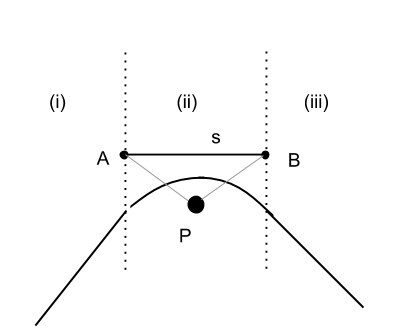
\includegraphics[width=7cm]{img/punkt-strecke.png}
\end{center}
\caption{Bisektor Punkt und Strecke}
\label{fig:c1}
\end{figure}

Betrachten wir nun die Bisektoren von zwei Strecken $s$ und $t$, dabei unterscheiden wir in (a) parallele Strecken und (b) nicht parallele Strecken.

\paragraph*{(a): parallele Strecken:}

\begin{itemize}
\item (1) $s$ und $t$ liegen auf einer Geraden (Spezialfall)
\item (2) überschneiden sich nicht
\item (3) überschneiden sich zum Teil oder ganz
\end{itemize}

Im Fall (2) und (3) entstehen 5 Bereiche:\\
(i) Gerade: Bisektor von den linkesten Punkten $A$ und $C$\\
(ii) Parabel: $s$ und $C$\\
(iii) Gerade: Gerade dazwischen\\
(iv) Parabel: $t$ und $B$\\
(v) Gerade: Bisektor von den rechtesten Punkten $B$ und $D$\\

\begin{figure}[h]
\begin{center}
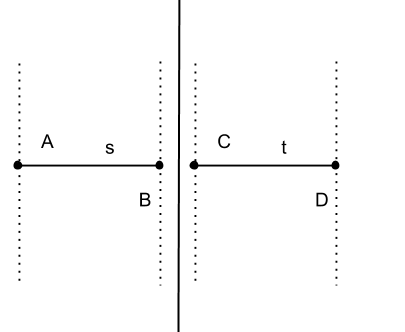
\includegraphics[width=7cm]{img/ssp1.png}
\end{center}
\caption{(1) Bisektor von zwei parallelen Geraden, auf einer Geraden.}
\label{fig:a1}
\end{figure}

\begin{figure}[h]
\begin{center}
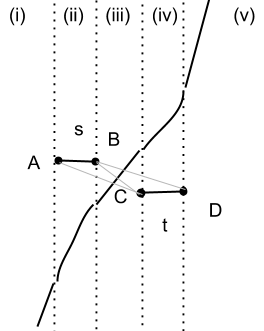
\includegraphics[width=7cm]{img/ssp2.png}
\end{center}
\caption{(2) Bisektor von zwei parallelen Geraden, keine Überschneidung.}
\label{fig:a2}
\end{figure}

\begin{figure}[h]
\begin{center}
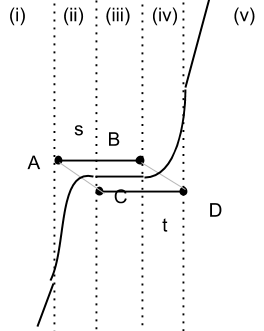
\includegraphics[width=7cm]{img/ss3.png}
\end{center}
\caption{(3) Bisektor von zwei parallelen Geraden, Überschneidung.}
\label{fig:a3}
\end{figure}

\begin{figure}[h]
\begin{center}
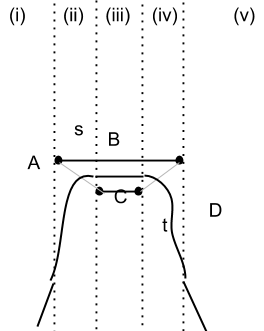
\includegraphics[width=7cm]{img/ss4.png}
\end{center}
\caption{(3) Bisektor von zwei parallelen Geraden, komplett innerhalb.}
\label{fig:a4}
\end{figure}

\paragraph*{(b): nicht parallele Strecken}

\begin{itemize}
\item (1) überschneiden sich nicht
\item (2) überschneiden sich zum Teil oder ganz
\end{itemize}

Hier entstehen im Fall (1) 4 Bereiche, im Falls (2) 7 Bereiche:\\

Erster Fall: wenn sie sich nicht überschneiden:\\
(i) Gerade\\
(ii) Winkelhalbierende\\
(iii) Parabel\\
(iv) Gerade\\

\begin{figure}[h]
\begin{center}
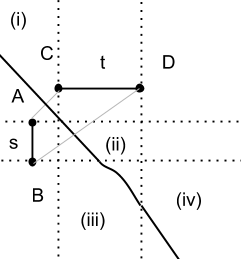
\includegraphics[width=7cm]{img/ssnpout.png}
\end{center}
\caption{(3) Bisektor von zwei nicht parallelen Geraden, keine Überschneidung.}
\label{fig:a5}
\end{figure}

Zweiter Fall: wenn sie sich überschneiden:\\
(i) Parabel\\
(ii) 2$\times$Winkelhalbierende\\
(iii) und (iv) Parabel\\
(v) Gerade\\
(vi) Parabel\\
(vii) Gerade\\

\begin{figure}[h]
\begin{center}
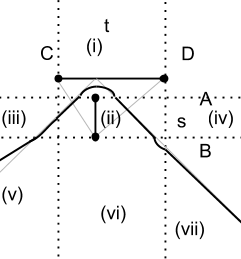
\includegraphics[width=7cm]{img/ssnpin.png}
\end{center}
\caption{(3) Bisektor von zwei nicht parallelen Geraden, mit Überschneidung.}
\label{fig:a5}
\end{figure}


Anzahl der Ecken: vielleicht wenn ich die Ecken weiß dann kommt man auch auf die Kanten.\\
Anzahl der Kanten: hm das weiß ich nicht.\\
Anzahl der Zellen: ist gleich Anzahl der Strecken.\\

Ich würde so wie bei den normalen Voronoi Diagrammen schauen was für Knoten es gibt und was die für einen maximalen Grad haben können und dann kann man das sicherlich irgendwie ausrechnen und die Kanten ergeben sich dann automatisch aus dem Gesamtdegree des Graphen oder so.


* Wie sehen die Voronoi-Kanten aus $\rightarrow$ Bilder von allen Fällen\\
* Aus wie vielen Ecken, Kanten und Zellen kann $VD(S)$ höchstens bestehen?\\
* Zeigen Sie dazu, dass die Voronoi-Regionen zusammenhängend sind.
\end{task}

\begin{task}{Fortune-Sweep}
\item[]
Die Sweepline sweept von links nach rechts, also entlang er $x$-Achse.

\begin{description}
\item[site] ist ein Punkt in der Ebene.
\item[beach line] teilt die Ebene in zwei Bereiche. Oberhalb der beach line sind alle Bereiche die potentiell zu den Voronoi Regionen der jeweiligen Punkte gehören werden. Unterhalb der beach line alle Punkte zu denen noch keine Aussage getroffen werden kann. Die Punkte auf der beach line sind equidistant zum zugehörigen Punkt und zur sweep line.
\item[spikes] zukünftige Voronoi Kanten. An Schnittpunkten von Spikes entstehen zukünftige Voronoi Knoten.
\item[breakpoint] sind die Schnittpunkte der Parabeln, dort befinden sich auch die Spikes, also durch die zwei Schnittpunkte verläuft genau ein Spike.
\item[site Event] tritt auf, wenn die Sweepline einen Punkt ("`site"') trifft.
\item[circle Event] tritt auf, wenn Kreisbögen verschwinden. D.h. ein circle event entsteht aus einem site event. Wenn sich zwei Spikes schneien, der Kreis durch die zugehörigen Punkte und dann ganz unten auf dem Kreis ist eine neues circle event.
\item[sweep line status (SLS)] enthält die Topologie der Beachline in Form einer Liste, sozusagen die Kreisbögen und die dazugehörigen Punkte und eine Information darüber, durch welches Event ein Kreisbogen verschwindet.
\item[event point schedule (EPS)] enthält site events und circle events. Die Priorität ist durch die $x$-Koordinate gegeben, d.h. tritt das Event weiter links auf, so ist die Priorität höher. Initialisiert wird die priority queue mit allen zu Beginn gegebenen Punkten.
\end{description}

Die Idee mit dem Binärensuchbaum leuchtet mir zwar ein, habe es aber nicht so doll verstanden, als dass ich es hier umsetzen könnte.


\paragraph*{Initialisierung}
\begin{description}
\item[EPS] $(0,0)[\text{se1}]$, $(1,2)[\text{se2}]$, $(2,3)[\text{se3}]$, $(4,3)[\text{se4}]$
\item[beachline] $\emptyset$
\end{description}

\paragraph*{EVENT 1 - site event $(0,0)$}
\begin{description}
\item[EPS] $(1,2)[\text{se2}]$, $(2,3)[\text{se3}]$, $(4,3)[\text{se4}]$
\item[beachline] $a_1 \rightarrow (0,0)$
\end{description}

\begin{figure}[h]
\begin{center}
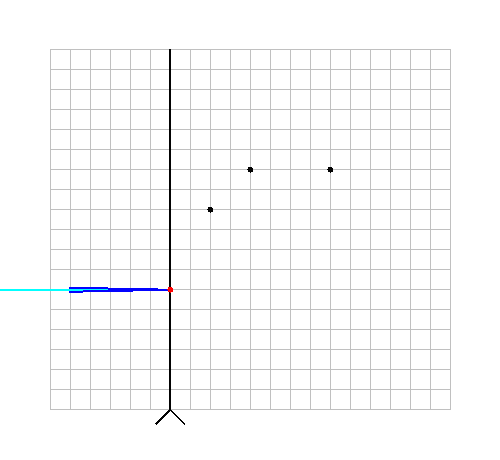
\includegraphics[width=7cm]{capture1}
\end{center}
\caption{Schritt 1}
\label{fig:c1}
\end{figure}

Keine circle event und keine neuen Kanten.

\newpage

\paragraph*{EVENT 2 - site event $(1,2)$}
\begin{description}
\item[EPS] $(2,3)[\text{se3}]$, $(4,3)[\text{se4}]$
\item[beachline]
$a_{1.1} \rightarrow (0,0)$,\\
$a_2 \rightarrow (1,2)$,\\
$a_{1.2} \rightarrow (0,0)$\\
\end{description}

\begin{figure}[h]
\begin{center}
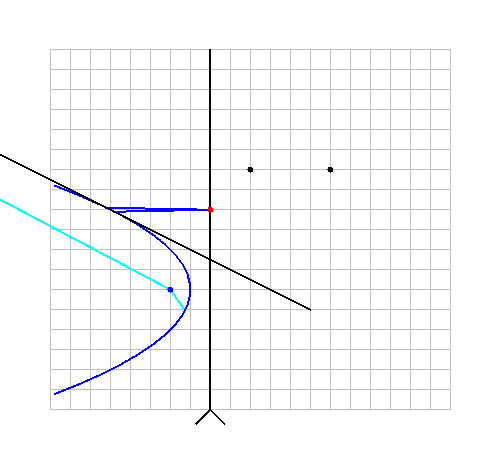
\includegraphics[width=7cm]{capture2}
\end{center}
\caption{Schritt 2}
\label{fig:c2}
\end{figure}

Keine circle event, zwei Spikes, werden noch zu Kanten, wenn die Position der Knoten bekannt ist.

\newpage

\paragraph*{EVENT 3 - site event $(2,3)$}
\begin{description}
\item[EPS] $(4,3)[\text{se4}], (11 + \sqrt{130}, -3)[\text{ce1}]$
\item[beachline]
$a_{1.1} \rightarrow (0,0)$\\
$a_{2.1} \rightarrow (1,2)$\\
$a_3 \rightarrow (2,3) [\text{delete at ce1}]$\\
$a_{2.2} \rightarrow (1,2)$\\
$a_{1.2} \rightarrow (0,0)$
\end{description}

\begin{figure}[h]
\begin{center}
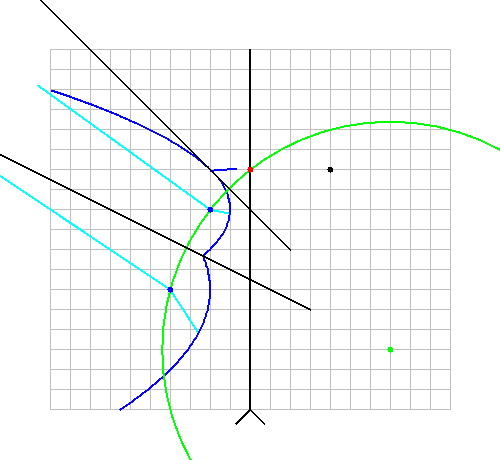
\includegraphics[width=7cm]{capture3}
\end{center}
\caption{Schritt 3}
\label{fig:c3}
\end{figure}

Der Schnittpunkt $(11, -3)$ der beiden Spikes ist ein evtl. zukünftiger Voronoi Knoten. Der Fußpunkt des grünen Kreises wird als neues circle event $(11 + \sqrt{130}, -3)[ce1]$ der EPS hinzugefügt.

\newpage

\paragraph*{EVENT 4 - site event $(4,3)$}
\begin{description}
\item[EPS] $(6 + \sqrt{20}, 2)[\text{ce2}], (7 + \sqrt{50}, -1)[\text{ce3}]$
\item[beachline]
$a_{1.1} \rightarrow (0,0)$\\
$a_{2.1} \rightarrow (1,2)$\\
$a_{3.1} \rightarrow (2,3)$\\
$a_4 \rightarrow (4,3)[\text{delete at ce2} (7 + \sqrt{50}, -1)]$\\
$a_{3.2} \rightarrow (2,3)$\\
$a_{2.2} \rightarrow (1,2)$\\
$a_{1.2} \rightarrow (0,0)$
\end{description}

Der Schnittpunkt der beiden letzen Spikes $(6,2)$ ist ein evtl. zukünftiger Voronoi Knoten. Der Fußpunkt dieses Kreises wird als neues circle event  $(6 + \sqrt{20}, 2)[\text{ce2}]$ der EPS hinzugefügt und rutsch in der priority queue ganz nach vorne.

Das alte circle event $(11 + \sqrt{130}, -3)$ wird aus der EPS gelöscht.

Der Schnittpunkt $(7, -1)$ des neuen Spikes und des Nachbarspike ist wieder in potentieller neuer Knoten im Voronoi Diagramm. Ein neues circle event kommt also hinzu $(7 + \sqrt{50}, -1)[\text{ce3}]$.

\begin{figure}[h]
\begin{center}
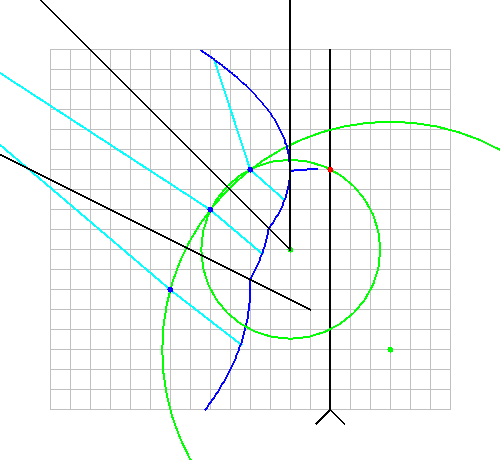
\includegraphics[width=7cm]{capture4}
\end{center}
\caption{Schritt 4}
\label{fig:c4}
\end{figure}

\newpage

\paragraph*{EVENT 5 - circle event $(6 + \sqrt{20}, 2)$}
\begin{description}
\item[EPS] $(7 + \sqrt{50}, -1)[\text{ce3}]$
\item[beachline]
$a_{1.1} \rightarrow (0,0)$\\
$a_{2.1} \rightarrow (1,2)$\\
$a_{3.1} \rightarrow (2,3)$\\
$a_4 \rightarrow (4,3)[\text{delete at ce3} (7 + \sqrt{50}, -1)]$\\
$a_{3.2} \rightarrow (2,3)$\\
$a_{2.2} \rightarrow (1,2)$\\
$a_{1.2} \rightarrow (0,0)$
\end{description}

\begin{figure}[h]
\begin{center}
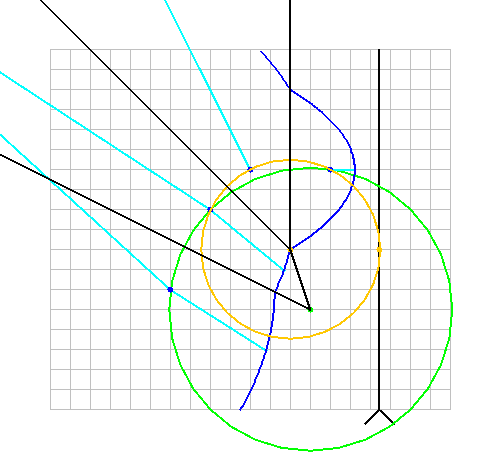
\includegraphics[width=7cm]{capture5}
\end{center}
\caption{Schritt 5}
\label{fig:c5}
\end{figure}

Ein Parabelbogen verschwindet, der Voronoi Knoten ist nun fest, sowie die beiden Voronoi-Kanten.

\newpage

\paragraph*{EVENT 6 - circle event $(7 + \sqrt{50}, -1)$}
\begin{description}
\item[EPS] $\emptyset$
\item[beachline]
$a_{1.1} \rightarrow (0,0)$\\
$a_{2.1} \rightarrow (1,2)$\\
$a_{3.1} \rightarrow (2,3)$\\
$a_{3.2} \rightarrow (2,3)$\\
$a_{2.2} \rightarrow (1,2)$\\
$a_{1.2} \rightarrow (0,0)$
\end{description}

\begin{figure}[h]
\begin{center}
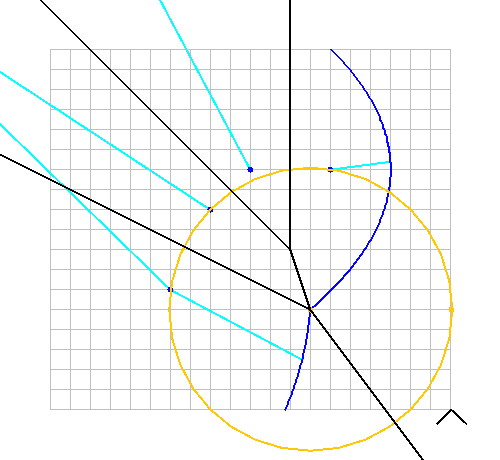
\includegraphics[width=7cm]{capture6}
\end{center}
\caption{Schritt 6}
\label{fig:c6}
\end{figure}

Ein Parabelbogen verschwindet, der Voronoi Knoten ist nun fest, sowie die beiden Voronoi-Kanten.

\newpage

\begin{figure}[h]
\begin{center}
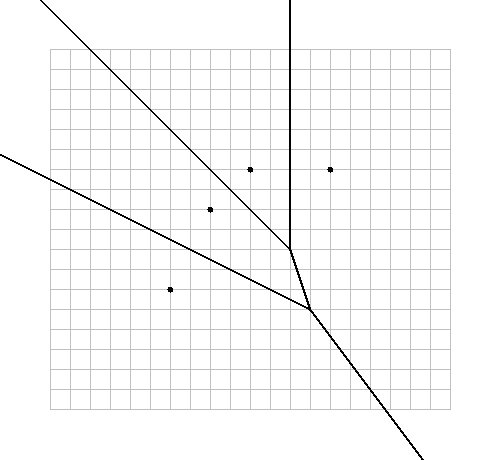
\includegraphics[width=7cm]{capture7}
\end{center}
\caption{Schritt 7}
\label{fig:c7}
\end{figure}

Am Ende muss erklärt werden, wie in einem Postprocessing mit Kanten verfahren wird, die nur an einem oder gar keinem Knoten hängen 



\end{task}

\begin{task}{Durchschnitt einfacher Polygone}
\item[]
Das Verfahren ähnelt ein wenig dem in der Vorlesung virgestellten zur Berechnung der Triangulierung einer Punktwolke mit einem Sweep-Line Verfahren: die Front besteht aus Intervallen die innerhalb von keinem, einem oder beiden Polygonen liegen. An Ereignispunkten werden Kanten des Schnitts hinzugefügt und Intervalle hinzugefügt/entfernt. Die bereits zu Beginn des Algorithmus bekannten Ereignispunkte sind die Koordinaten der Ecken der Polygone (Punktereignisse), die dynamischen Ereignispunkte sind Schnittpunkte zwischen Kanten der beiden Polygone (Schnittereignisse).

Es ist viel anschaulicher (wirklich :) ) und rechnet sich oft leichter (siehe Parabeln bei Fortune) die Sweepline ''von oben nach unten'' laufen zu lassen und die Front ''von links nach rechts'' zu organisieren. Als totale Ordnung der Punkte der Ebene sei hier deshalb eine Sortierung vorgeschlagen, die zunächst absteigend nach Y-Koordinate und danach aufsteigend nach X-Koordinate sortiert.

Es seien im Folgenden $P=(V_p,E_p),R=(V_q,E_q)$ zwei Polygone für die $S=P\cap Q$ berechnet werden soll. Benötigt werden auch hier eine Prioritätswarteschlange $Q$ und eine geeignete Datenstruktur (z.B. binärer Suchbaum) um die Front $F$ zu verwalten.

Ein Intervall $i=(l,r,e_l,e_r,o)$ besteht aus Verweisen $l$/$r$ auf das linke/rechte Nachbar-Intervall, den Kanten $e_l$/$e_r$ die das Intervall nach links/rechts abgrenzen (eine würde reichen, beide zu haben erleichert aber das Aufschreiben ...) und einem Hinweis $o\in\{ 0,P,Q,S\}$ ob das Intervall zu keinem Polygon / nur $P$ / nur $Q$ / $S$ gehört.

Für ein Schnittereignis $s=(p,e_l,e_r)$ werden neben der Position $p$ an der es auftritt auch die Kanten $e_l,e_r$ gespeichert, die sich geschnitten haben.

Algorithmus:\\
(1) Füge alle Ecken aus $P,R$ zur Prioritätswarteschlange $Q$ hinzu\\
(2) Solange $Q$ nicht leer ist: bearbeite \& entferne das erste Ereignis aus $Q$\\
(3) Gebe Ergebnis $S$ zurück

Mit Punktereignissen bzw. Schnittereignissen wird nun wie folgt verfahren:

Punktereignis $p$:\\
Zu $p$ gehören stets zwei ausgehende Kanten $e_1=(p,(x_l,y_l)),e_2=(p,(x_r,y_r))$ wobei $x_l<x_r$, sowie ein Polygon $P(p)$.\\
(P1) Suche das Intervall $i=(l,r,e_l,e_r,o)$ in $F$, für das die X-Koordinate von $p$ zwischen den X-Koordinaten der Knoten von $e_l,e_r$ liegt, welche die größere Y-Koordinate haben.\\
(P2): Prüfe ob ein Schnittpunkt $s$ zwischen $e_1$ und $e_l$ existiert. Wenn ja, setzte $e_1=(p,s)$ und füge das Schnittereignis $e=(s,e_l,e_1)$ zu $Q$ hinzu.\\
Es muss ebenfalls geprüft werden, ob ein Schnittpunkt zwischen $e_1$ und $e_r$ existiert. Ebenso müssen Schnitte mit $e_2$ berücksichtigt werden - in allen Fällen wird analog verfahren.\\
(P3):
\begin{itemize}
\item Fall 1: $F$ ist leer\\
Füge zu $F$ das Intervall $j=(null,null,e_1,e_2,P(p))$ hinzu
\item Fall 2: Die Endpunkte von $e_1$ und $e_2$ liegen beide unterhalb von $p$:\\
Dann wird $i$ aufgespalten und ein neues Intervall $j=(i,i,e_1,e_2,o_j)$ zwischen die aufgespaltenen Teile eingefügt (Zeiger werden entsprechend umgelegt).
$$o_j=\begin{cases}
0&\text{, falls }o=P(p)\\
P(p)&\text{, falls }o=0\\
S&\text{, sonst} 
\end{cases}$$
Falls $o_j=S$ werden $e_1,e_2$ mit den dazugehörigen Kanten zu $S$ hinzugefügt.
\item Fall 3: Die Endpunkte von $e_1$ und $e_2$ liegen beide oberhalb von $p$:\\
Dann wird der Polygonzug an dieser Stelle geschlossen. Falls $o_j=S$ werden $e_1,e_2$ mit den dazugehörigen Kanten zu $S$ hinzugefügt. $i$ wird aus $F$ entfernt und $l$ mit $r$ vereinigt (es sollten bzgl. der Polygonzugehörigkeit hier keine Uneindeutigkeiten auftreten). Für die begrenzenden Kanten des vereinigten Intervalls muss nun erneut auf Schnittereignisse geprüft werden.
\item Fall 4:\\
Es handelt sich um eine ''Durchgangskante''. Die Kante $e\in\{ e_l,e_r\}$ die mit $p$ verbunden ist wird durch die ''nach unten zeigende'' Kante ersetzt. Es muss auf Schnittereignisse geprüft werden und falls $o=S$ die neue Kante zu $S$ hinzugefügt werden.
\end{itemize}

Schnittereignis $s$:\\
(S1): Es wird verfahren wie bei (P1)-(P3), wobei $e_1,e_2$ die Kanten sind, bei denen ein Endpunkt eine kleinere Y-Komponente hat als $s$. In (P3) greift somit Fall 2 - es unterscheidet sich hier nun aber die Belegung von $o_j$:
$$o_j=\begin{cases}
0&\text{, falls }o=S\\
S&\text{, falls }o=0\\
P&\text{, falls }o=Q\\
Q&\text{, sonst} 
\end{cases}$$

Zeitkomplexität:\\
\begin{itemize}
\item Sortieren in (1) benötigt $O(n\cdot\log n)$
\item Jeder Schnittpunkt zwischen $P$ und $R$ ist immer auch Ecke von $S$ (Berührpunkte zählen nicht als Schnitt). Es gibt insgesamt also genau $k$ Schnittereignisse. Die Schleife in (2) wird folglich $\Theta (n+k)$ mal ausgeführt.
\item Jedes Mal wenn ein Intervall zur Front hinzugefügt wird, wird ein bestehendes aufgespalten. Im entarteten Fall kann dies $O(n+k)$ mal erforderlich sein, es können also maximal $2\cdot (n+k)$ Elemente in $F$ vorhanden sein. Steht für $F$ eine passende DS (Baum) zur Verfügung, kann somit bei (P1) in $O(\log (n+k))$ gesucht werden (amortisiert vermutlich besser).
\item (P2) kann $O(\log (n+k))$ erfordern, um neue Ereignisse einzusortieren.
\item (P3) kann $O(\log (n+k))$ erfordern, um neue Intervalle abzulegen.
\end{itemize}
$$\rightarrow O((n+k)\cdot\log (n+k))$$
\end{task}
\end{document}